\documentclass[a4paper, 12pt, oneside]{report}

% \title{First document}
% \author{Huy Nhat Minh Nguyen}
% \date{May 2022}
%%%%%%%%%%%%%%%%%%%%%%%%%%%%
% LINE SPACING
\newcommand{\linespacing}{1.5}
\renewcommand{\baselinestretch}{\linespacing}
%%%%%%%%%%%%%%%%%%%%%%%%%%%%
\setlength{\headheight}{14.5pt}

%%%%%%%%%%%%%%%%%%%%%%%%%%%%
% BIBLIOGRAPHY STYLE
\usepackage{natbib}
% \bibliographystyle{plain} for [1], [2] etc.
% \bibliographystyle{apalike}
%%%%%%%%%%%%%%%%%%%%%%%%%%%%


%%%%%%%%%%%%%%%%%%%%%%%%%%%%
% OTHER FORMATTING/LAYOUT DECLARATIONS
\usepackage{amsmath}
\usepackage{longtable}
\usepackage{setspace}
\usepackage{standalone}

% The left-hand-side should be 40mm.  The top and bottom margins should be
% 25mm deep.  The right hand margin should be 20mm.
\usepackage[a4paper,top=3cm,bottom=3cm,left=3cm,right=3cm,headsep=10pt]{geometry}
\flushbottom
% Pages should be numbered consecutively through the main text.  Page numbers
% should be located centrally at the top of the page.
\usepackage{fancyhdr}
\fancypagestyle{plain}{
	\fancyhf{}
	% Add "DRAFT: <today's date>" to header (comment out the following to remove)
	%\lhead{\textit{DRAFT: \today}}
	%
	\chead{\thepage}
	\renewcommand{\headrulewidth}{0pt}
}
\pagestyle{fancy}
%%%%%%%%%%%%%%%%%%%%%%%%%%%%

% HYPERREF
\usepackage[colorlinks,pagebackref,pdfusetitle,urlcolor=blue,citecolor=blue,linkcolor=blue,bookmarksnumbered,plainpages=false]{hyperref}
% For print version, use this instead:
%\usepackage[pdfusetitle,bookmarksnumbered,plainpages=false]{hyperref}
%\usepackage{backref}
%\renewcommand{\backrefpagesname}{Cited on}
%%%%%%%%%%%%%%%%%%%%%%%%%%%%


%%%%%%%%%%%%%%%%%%%%%%%%%%%%
% BEGIN DOCUMENT
\begin{document}
%%%%%%%%%%%%%%%%%%%%%%%%%%%%


%%%%%%%%%%%%%%%%%%%%%%%%%%%%
% PREAMBLE: roman page numbering i, ii, iii, ...
\pagenumbering{roman}
%%%%%%%%%%%%%%%%%%%%%%%%%%%%


%%%%%%%%%%%%%%%%%%%%%%%%%%%%
%% TITLE PAGE: The title page should give the following information:
%%	(i) the full title of the thesis and the sub-title if any;
%%	(ii) the full name of the author;
%%	(iii) the qualification aimed for;
%%	(iv) the name and logo of the University;
%%	(v) the month and year of submission.
\thispagestyle{fancy}
\begin{flushright}
\includegraphics[width=8cm]{Images/uts_logo_complete.jpg}
\end{flushright}	
\vskip20mm
\begin{center}
% TITLE
\LARGE\textbf{Extrinsic calibration of multiple partially overlapping RGB-D cameras}
\vskip5mm
% SUBTITLE (optional)
\large\textit{Capstone Thesis}
\vskip2mm
% AUTHOR
\normalsize\textbf{Huy Nhat Minh Nguyen}

\vspace{20mm}
\normalsize
Student Number: 13734569 \\
Project Number: AUT-22-07822 \\
Major: Mechatronics Engineering
\vskip5mm
Supervisor: Dr. Alen Alempijevic \\
Co-Adviser: Mr Jasprabhjit Mehami \\
% \normalsize
\end{center}
\vfill
\begin{center}
\normalsize
% QUALIFICATION
41030 - Engineering Capstone \\
Bachelor of Engineering (Honours) \\
University of Technology Sydney	\\
Faculty of Engineering and Information Technology\\
% DATE OF SUBMISSION
31 May, 2022
\end{center}
%%%%%%%%%%%%%%%%%%%%%%%%%%%%


%%%%%%%%%%%%%%%%%%%%%%%%%%%%
% SUMMARY PAGE
\chapter*{Author's declaration}
% \begin{SingleSpace}
\begin{quote}
I, 
\emph{Huy Nhat Minh Nguyen} declare that this thesis, submitted in fulfilment of the requirements for the Bachelor of Engineering (Honours) in the
\emph{School of Mechanical and Mechatronic Engineering}, 
\emph{Faculty of Engineering and Information Technology}
at the University of Technology Sydney, Australia, 
is wholly my own work unless otherwise referenced or acknowledged. 
In addition, I certify that all information sources and literature used are indicated in the thesis.
This document has not been submitted for qualifications at any other academic institution.

\vspace{1.5cm}
\noindent 
\hspace{-0.75cm}\textsc{Signature: } \underline{
~~~~~~~~~~~~~~~~~~~~~~~~~~~~~~~~~~~~~~~~~~~~~~~~~~~~~~~~~~~~~~~~
}


\noindent
\hspace{-0.75cm}{~~~~~~~~~~~~~~~~~~~~~~~~[Minh Nguyen]}\\

\noindent 
\hspace{-0.75cm}\textsc{Date: } 30\textsuperscript{th} May, 2022

\noindent 
\hspace{-0.75cm}\textsc{Place: } Sydney, Australia



\end{quote}
% \end{SingleSpace}
\clearpage
\thispagestyle{fancy}
\null\vskip10mm
\begin{center}
\underline{\textsc{Abstract}}
\vskip2mm
\end{center}
% Change line spacing
\renewcommand{\baselinestretch}{1.0}
\small\normalsize
% Abstract HERE (300 word limit for most subjects):
Exteroceptive sensors and cameras have been widely implemented in various engineering fields, especially in robotics and vision. Working with a camera or a multiple camera system requires accurate camera parameters, including the intrinsic and extrinsic parameters. This led to the introduction of different camera calibration methods with varying calibration targets, depending on specific camera types and project purposes.

Planar calibration targets have been extensively applied in multiple camera system calibration methods due to their simple implementation, high precision and cheap production, compared with 3D calibration targets. However, in working with calibrating a system with numerous cameras, some planar calibration targets reveal certain inconveniences, especially for extrinsic calibration. For example, in a system with multiple cameras facing each other, all cameras cannot completely capture the planar calibration target. This limits the application of the calibration method using planar calibration target to various camera system configurations.

This capstone project proposes a method using an augmented planar calibration target to calibrate a multiple partially overlapping RGB-D camera system. A double-sided planar board is employed to avoid the limitations of planar targets, and the ArUco marker system is adopted as fiducial marker to support the detection algorithm. In addition, this calibration method applies the General Graph Optimisation (G2O) framework to optimise and guarantee the accuracy of the extrinsic parameters during the calibration process. This project experimentally validates the method's accuracy and discusses the applicability of the proposed technique. Finally, this project provides the framework's source code and supporting documentation, which is mainly programmed in C++ and MATLAB with ROS as a middle-ware, for further use and development.


% %%%%%%%%%%%%%%%%%%%%%%%%%%%%
% ACKNOWLEDGEMENTS
\newpage
\section*{Acknowledgments}

\renewcommand{\baselinestretch}{\linespacing}
\small\normalsize
% ACKNOWLEDGEMENTS HERE:
This capstone project as well as the thesis would not be successful without the instruction and assistance of the people around me. I would particularly like to acknowledge:

\vspace{10mm}
Special thanks to Dr Alen Alempijevic, my supervisor, for being supervised this capstone project. His mentorship and guidance is the role key of the success of this project. It is my honour to have the opportunity to work with him.

\vspace{10mm}
Mr Jasprabhjit Mehami, for following me closely and helping me throughout the process of working on the project. His knowledge and experience in camera and vision contributed greatly to the success of this approach.

\vspace{10mm}
My family and loved ones, for being always by my side to support me mentally, helping me to always feel comfortable and confident to complete this capstone project as well as the thesis.

\vspace{10mm}
My friends in Australia, for their support whenever I encountered a struggle during the process of doing this capstone project.



%%%%%%%%%%%%%%%%%%%%%%%%%%%%
% TABLE OF CONTENTS, LISTS OF TABLES & FIGURES
\pdfbookmark[0]{Contents}{contents_bookmark}
\tableofcontents
\listoftables
\phantomsection
\addcontentsline{toc}{chapter}{List of Tables}
\listoffigures
\phantomsection
\addcontentsline{toc}{chapter}{List of Figures}
%%%%%%%%%%%%%%%%%%%%%%%%%%%%


%%%%%%%%%%%%%%%%%%%%%%%%%%%%
% MAIN THESIS TEXT: arabic page numbering 1, 2, 3, ...
\newpage
\pagenumbering{arabic}

%-----------------------------------------------------
% Chapter: Introduction
%-----------------------------------------------------

% NB Good idea to put each chapter in a separate file.
% If you put the following in a file called "thesis_introduction.tex"
% then you can include it with the following:

\lhead{}

\chapter{Introduction}

\section{Project background}

This thesis was completed in synergy with the "Objective real-time live cattle assessments to improve profit" funded project by Meat and Livestock Australia. The overarching project aims to develop and improve profitability and productivity of the beef value chain, addressing cattle non-compliance with processor grid specifications – a \$51M pa issue for the sector and more when feeding costs are taken into consideration. This problem is aggravated by the failure to improve production efficiencies because data on cattle traits is unavailable in real-time. The industry opportunity is to have an objective real-time assessment of live cattle to assist producers to achieve greater production efficiencies by meeting "market specifications" and increasing lean meat yield so that additional dollars flow into producers' pockets.

The project has developed bespoke designed inserts for a race that ensure cattle can move freely, is safe and provides unobstructed views of cattle from multiple RGB-D cameras. We have created a software framework that enables measuring hip height and estimating P8 fat and Muscle Score. To effectively perform this software framework, a thoroughly calibrated 3D multiple-cameras system is strongly required. A calibrated multiple-cameras system would provide specific parameters of cameras to operate involved tasks. 

Camera parameters included intrinsic parameters and extrinsic parameters, combined to define the mathematical relationship between 3D global points $P(X, Y, Z)$ and their corresponding 2D image plane points $p(u, v)$. The intrinsic parameters, also known as the camera matrix, belong to the camera itself, consisting of the focal length f, the principal point (the optical centre), and the lens distortion. Each camera has unique intrinsic parameters that come from the physical design process. The extrinsic parameters, or the camera pose, are used to illustrate the geometrical relationship (rotation and translation) between the camera itself and a feature in its external world \citep{Zhang2014}. Specifically, in this project's scope, the extrinsic parameters of a multiple-camera system are the transformation relationship between each camera and others in this structure.

Nowadays, camera calibration is essential for any computer vision system. Several software toolboxes and packages are provided and widely adopted to simplify the calibration process as well as ensure the accuracy of the results, the most common being the Open-CV library or the MATLAB Computer Vision Toolbox. However, in particular multiple-camera systems, such as the multiple partially overlapping cameras system, conventional methods cannot be used for accurate parameter results.

This capstone report focus on researching and implementing a method for multiple partially overlapping RGB-D cameras calibration compatible with the ROS framework in C++ programming language. The approach is expected to solve the problem of extrinsically calibrating the camera system with fields of view overlapping and facing each other that cannot be handled using standard calibration methods.

\section{Project scope}
This capstone project proposes to use a double-sided ArUco board as the calibration target, with the support of the Open-CV library and the General Graph Optimisation (G2O) framework \citep{Kummerle2011}. The software included with this method is implemented mainly in C++ and MATLAB, and ROS (Robot Operating System) is used as a middle-ware to transfer data between the program and the multiple-camera system.

\section{Thesis outline}
This capstone thesis is structured as follows:

Chapter 2 looks at the literature review of the previous camera calibration relevant to this project's purpose. This chapter evaluates the advantages and drawbacks of these methods, as well as considers the possibility and suitably to the project's objectives. It also explains why specific project decisions were taken.

Chapter 3 presents the approach and the methodology of this project. These ideas are described and explained in detail. This chapter also provides important insights necessary to understand the work of the project.

Chapter 4 demonstrates the implemented experiments to check the possibility and efficiency of the approach. The implementation, relevant equipment and results obtained are described in detail. 

Chapter 5 discusses the methodology as well as the experiments implemented. This chapter reviews the accuracy of experimental results, clarifies the uncertainties and difficulties of this approach, and plans potential future works to improve this method.

\chapter{Literature Review}
With the development of science and technology, computer vision has gradually become popular in various engineering fields, leading the demand for exteroceptive sensors to increase in many different applications. In order to work with cameras, calibration is a critical stage and must be completed before capturing data \citep{Baker2003}. Therefore, various camera calibration methods have been published, suited to different project purposes. 

This chapter aims to provide a literature review of the previous camera calibration methods and discuss both the benefits and drawbacks of these methods. These related works are considered and analysed thoroughly to determine the most suitable approach for our project purpose.


\section{Camera calibration}
The actual camera calibration process is performed using calibration targets. These targets have a definite structure or sample, and their geometry is known for great precision. The camera will take the image of these calibration targets and then calculate the camera parameters (intrinsic and extrinsic) using math formulas and algorithms. One of the most notable publications on camera calibration is by \cite{Tsai1987}; he presented a two-stage camera calibration method using a mono view co-planar set of points. \cite{Zhang2000} proposed a calibration method using Closed-Form solution and Maximum-Likelihood Estimation. In this approach, his calibration target was a planar board with mostly square patterns and circle patterns at the corners, printed on paper and stuck onto the board. Research by \cite{Triggs1999} showed that the camera is required to capture at least five 3D points to one image to calibrate the extrinsic parameters. There is a drawback in Triggs' approach that these five 3D calibration dots had to belong to at least two different planes. 

\section{Multi-camera calibration}

\subsection{Stereo cameras}
Unlike calibrating a single camera, the calibration technique for a system with several cameras is more complicated and troublesome. In this situation, the intrinsic parameters must be calibrated independently, while the extrinsic calibration process should be implemented simultaneously. Various calibration methods have been published to estimate the extrinsic parameters of a multiple camera system. In research in 2003, Tomita and Ueshiba introduced a calibration method for two cameras using a planar calibration target. This pair of cameras would capture images of the target from two different orientations. Then, applying homography, both cameras would be intrinsically and extrinsically calibrated, and all the camera parameters would be solved \citep{Ueshiba2003}. With this method, although capturing images from two different orientations is enough, we can improve the accuracy of the calibration process by capturing more images from various locations. This method was then developed by calibrating a system with twelve cameras precisely.

\begin{figure}[ht]
\centering
\includegraphics[width=0.7\textwidth]{Images/Tomita.png}
\caption{Ueshiba \& Tomita (2003) calibration method for overlapping camera system}
\end{figure}

\subsection{Non-overlapping Field of View cameras}
However, the calibration method of Tomita \& Ueshiba contained a significant drawback. This approach only works with a multiple overlapping camera system, which means all the cameras in the system have to be able to capture the 2D calibration target fully. In a research in 2016, \cite{Dong2016} introduced a method to calibrate a non-overlapping camera system. He used a wide planar board and printed encoded patterns with predefined positions (relative to the board origin). Therefore, each camera in the system does not need to capture the whole board during calibration, and camera can identify every single encoded pattern using a binary color-coding system. However, this method can only apply to extrinsically calibrate the camera system, so Dong had to get the intrinsic parameters of his cameras using Zhang's method.

\begin{figure}[ht]
\centering
\includegraphics[width=0.8\textwidth]{Images/Dong (2016).jpg}
\caption{Dong et al. (2016) method for non-overlapping multiple camera system}
\end{figure}

Dong's calibration method still requires the cameras are placed close together with the same orientation due to the particular characteristics of the 2D calibration target. In fact, depending on the project purpose, there will be cases where the system contains cameras facing each other, and 2D calibration targets cannot be used because all cameras cannot thoroughly capture the planar calibration target. \cite{Marcon2017} introduced a calibration method that used a double-sided checkerboard. The cameras having opposite orientations independently capture one side of the board, and then the extrinsic parameters are estimated together with the displacement error between two sides of the board.

\begin{figure}[ht]
\centering
\includegraphics[width=1\textwidth]{Images/Marcon (2017).png}
\caption{Double-sided checkerboard of Marcon et al. (2017)}
\end{figure}

However, Marcon's (2017) approach could not solve the problem of cameras facing back to each other, for example, the airborne remote sensing camera system. Therefore, \cite{Yin2018} proposed a calibration method as a solution for these multi-camera systems. In his approach, he chose one camera as the origin reference frame, and then the extrinsic parameters would be the relative pose between each camera in the system to the reference camera. His method consisted of two stages: estimating the relative poses between every pair of cameras in this system and then calculating the extrinsic parameters based on optimising the re-projection errors using the Global Optimal Method. The results obtained were very positive: 0.001 radians and 0.08 millimetres on rotation and translation, respectively.

\begin{figure}[ht]
\centering
\includegraphics[width=0.9\textwidth]{Images/Yin et al. (2018).png}
\caption{Yin et al. (2018) calibration method}
\end{figure}

\clearpage
Additionally, several calibration methods use non-planar calibration targets or 3D calibration objects. \cite{Shen2011} published a technique using a sphere to calibrate a multi-camera system. They used eight 3D calibration dots, which are spherical with different colors, for the calibration of a system with twelve cameras. In this approach, each camera does not need to capture all eight dots in the calibration process, because just six calibration points are required to be captured by each camera once.



\begin{figure}[ht]
\centering
\includegraphics[width=1\textwidth]{Images/Shen (2011).png}
\caption{Spherical calibration targets of Shen \& Hornsey (2011)}
\end{figure}

\clearpage
\section{Fiducial markers}
Fiducial markers play an essential role in camera calibration. Fiducial marker defines visual sample targets within a physical environment that is discoverable and localisable by kinds of an exteroceptive sensor (camera, lidar...) \citep{Korthals2019}. Numerous types of fiducial markers were proposed in computer vision systems, such as ArUco markers \citep{Garrido-Jurado2014}, AprilTag \citep{Olson2011}, ARToolKit... Fiducial markers have been widely used in various vision applications, including camera calibration, robotics and augmented reality. Moreover, many support libraries have been provided to simplify the adoption of these markers.

\begin{figure}[ht]
\centering
\includegraphics[width=1\textwidth]{Images/Fiducial markers.jpg}
\caption{Fiducial markers}
\end{figure}

\clearpage
\section{General Graph Optimisation}
To increase the accuracy of camera parameters during the calibration process, especially calibrating a multi-camera system, we should repeat the calibration procedure many times to optimise the result. The problem of graph optimisation has been researched extensively in several computer vision and robotics fields. \cite{Reinke2019} have proposed an extrinsic calibration method for a multi-camera system on legged robots based on factor graph optimisation. In their experiments, they captured a total of 1312 images, and after calibrating, their results had errors of about 2.03\% and 3.8\% on translation and rotation, respectively.

\begin{figure}[ht]
\centering
\includegraphics[width=0.8\textwidth]{Images/Reinke et al. (2019).png}
\caption{Multiple camera system on a legged robot}
\end{figure}

\chapter{Approach}

This capstone report aims to develop a method to calibrate the extrinsic parameters of a multiple partially overlapping RGB-D camera system. Each camera in the system already has the intrinsic parameters (from the manufacturer), so this report just focuses on extrinsically calibrating. The approach consists of two main parts: the first section proposes the double-sided ArUco board as the calibration target and estimates the relative pose between the board and each camera in the system, and the second part mentions the application of the General Graph Optimisation in our method.

\clearpage
\section{Camera model}
% The expected rate of events is $\lambda$. 

It is essential to obtain a good established mathematical modelling that correctly defines the operating of a typical camera to handle the calibration. In this method, the pinhole camera model is used to describe a 3D point $P(X, Y, Z)$ in the global frame to a 2D image plane position $p(u, v)$ via a projection matrix $M$.
\[
s
\begin{bmatrix}
    u \\
    v \\
    1
\end{bmatrix}
=M
\begin{bmatrix}
    X \\
    Y \\
    Z \\
    1
\end{bmatrix}
\]

The projection matrix $M$ combines the intrinsic parameters $K$ and the extrinsic parameters $[R, T]$ for a camera in a specific setup.
\[
M=K[R T]
\]

To determine the relative pose between cameras in the system (also known as the extrinsic parameters), firstly, we have to estimate the transformation from the calibration target (in this case is the ArUco board) to each camera. To optimise the calibration result, this work is performed continuously throughout the calibration process. All the transformation (translation and rotation) between the cameras to the ArUco board during the calibration process are recorded for the Pose Graph Optimisation.

The Perspective-n-Point (PnP) pose computation problem is reviewed to detect the ArUco board pose respected to the camera frame. This method estimates the relative transform (translation and rotation) between a calibrated camera (with all the intrinsic parameters) and a 3D target, minimising the re-projection error from the 2D-3D point.
\clearpage

\begin{figure}[ht]
\centering
\includegraphics[width=1\textwidth]{Images/Perspective-n-Point (PnP) pose problem.jpg}
\caption{Perspective-n-Point (PnP) pose problem}
\end{figure}

Theoretically, we have a set of 3D points within a global frame of reference and their respective 2D image projections. Assuming the camera has been intrinsically calibrated already and the camera matrix is defined, we are able to determine the relative pose (position and orientation) between the camera itself and the global frame. This follows the projecting model in perspective for the cameras:
\[
p_{I}=K[RT]p_{W}
\]
In which:

$p_{W}=[X_{W}, Y_{W}, Z_{W}, 1]$: the global point coordinates in homogeneous form.

$p_{I}=[u,v,1]$: the respective image point coordinates in homogeneous form.

$
K=
\begin{bmatrix}
    f_{x} &  0      & c_{x} \\
    0     &  f_{y}  & c_{y} \\
    0     &  0      & 1
\end{bmatrix}
$
a matrix includes the intrinsic parameters, also known as camera matrix. $f_{x}$, $f_{y}$ is the focal length and $c_{x}$, $c_{y}$ is the principal point.

$R, T$: 3D rotation and translation matrix (extrinsic parameters).

This results in the formula equation of the model:
\[
\begin{bmatrix}
    u \\
    v \\
    1
\end{bmatrix}
=
\begin{bmatrix}
    f_{x} &  0      & c_{x} \\
    0     &  f_{y}  & c_{y} \\
    0     &  0      & 1
\end{bmatrix}
\begin{bmatrix}
    r_{11} &  r_{12} & r_{13} & t_{x} \\
    r_{21} &  r_{22} & r_{23} & t_{y} \\
    r_{31} &  r_{32} & r_{33} & t_{z} \\
    0      &  0      & 0      & 1
\end{bmatrix}
\begin{bmatrix}
    X_{W} \\
    Y_{W} \\
    Z_{W} \\
    1
\end{bmatrix}
\]

Therefore, the relative pose combines the 3D translation and the 3D rotation, which transforms a 3D object in the global frame into the camera frame:
\[
\begin{bmatrix}
    X_{C} \\
    Y_{C} \\
    Z_{C} \\
    1
\end{bmatrix}
=
\begin{bmatrix}
    r_{11} &  r_{12} & r_{13} & t_{x} \\
    r_{21} &  r_{22} & r_{23} & t_{y} \\
    r_{31} &  r_{32} & r_{33} & t_{z} \\
    0      &  0      & 0      & 1
\end{bmatrix}
\begin{bmatrix}
    X_{W} \\
    Y_{W} \\
    Z_{W} \\
    1
\end{bmatrix}
\]

\clearpage
\section{Calibration target configuration: double-sided ArUco board}
We propose a double-sided planar board configuration with a set of ArUco markers as the calibration target. The board's thickness is carefully measured to the nearest 0.1 millimetres. The ArUco markers are printed on paper and mounted on both sides of the board, following the given order. These markers are the same size with given side lengths. In addition, to simplify the detection process, the $[x, y, z]$ coordinates of 4 corners of the ArUco markers are determined, which is respected to the board's origin frame. Finally, the origin coordinate frame of the double-sided board is identified in the lower-left corner of the front side of the board.
\vspace{5mm}

\begin{figure}[ht]
\centering
\includegraphics[width=1\textwidth]{Images/ArUco board configuration.png}
\caption{ArUco double-sided board configuration}
\end{figure}

\clearpage
\section{Pose Graph Optimisation}

We propose creating a pose graph, as shown in Figure \ref{fig:posegraph}. The pose graph consists of nodes that are connected by edges, which determines the relative pose between any two corresponding nodes in the graph and can contain uncertainty information of the measurement. The white nodes $X_{k}, k \in \{1,2,..., M\}$ denote the cameras in our system, and the grey nodes $L_{i}, i \in \{1,2,..., N\}$ represent the double-sided ArUco board's origin poses that are detected by at least two cameras. Note that the board pose does not need to be detected by all cameras. Therefore, in the graph each board pose node (grey) must be connected with at least two camera nodes (white), with the edges being the relative poses between the board's origin and the corresponding camera.


\begin{figure}[ht]
\centering
\includegraphics[width=1\textwidth]{Images/pose graph.png}
\caption{Pose Graph represents the calibration method}
\label{fig:posegraph}
\end{figure}

\chapter{Evaluation and Results}
This chapter describes the experimental process of this camera calibration method and the equipment used for the experiments. Furthermore, all the system parameters and results are also demonstrated in detail. Even though the system contains 16 cameras, we worked with four cameras in this experiment scope to test the calibration method. If the experiment result is accurate, we will gradually increase the number of cameras for further experiments.

\clearpage
\section{Overview}
Firstly, this chapter mentions the equipment necessary for the experiment, especially the cameras and the double-sided ArUco board. Cameras with their intrinsic parameters, as well as the ArUco board configuration, are defined clearly. 

This chapter then demonstrates the extrinsic calibration process for each camera. In order to optimise the calibration result, each camera continuously captures the image of the ArUco board and estimates the board's transformation respecting to the camera frame during the calibration process.
Finally, the set of estimated board poses of the whole camera system from the previous stage is processed by the General Graph Optimisation (G2O) framework. This framework aggregates the detected board's poses of the entire procedure and then calculates the final extrinsic parameters between cameras in the system.

This experiment's program framework and algorithm are mainly programmed in C++ with Open-CV 4.2.0 library. MATLAB programming language is also used to test the algorithm and initialise the ArUco board configuration. Besides, we use ROS Noetic as a middle-ware to help communicate between the camera system and our framework.

\clearpage
\section{Camera system}
For the scope and purpose of this experiment, we decide to use four RGB-D cameras Intel Realsense RGB-D D435i. This type of camera can capture images up to 1920x1080 resolution with a frame rate up to 60 Hz. The RGB-D camera can also capture depth images, which is very important for our project purpose, such as 3D reconstruction. Furthermore, the manufacturers have calibrated the intrinsic parameters of these cameras, so we just have to focus on the extrinsic calibration problem. Additionally, these cameras can be synchronised together via cable, which is important in working with multiple cameras. Intel has developed a ROS "wrapper" for the camera firmware that makes it more straightforward to communicate between the cameras and our framework, simplifying the programming for the calibration algorithm.

\begin{figure}[ht]
\centering
\includegraphics[width=0.9\textwidth]{Images/Realsense.jpg}
\caption{RGB-D Camera Intel Realsense D435i}
\end{figure}

The intrinsic parameter (also known as the camera matrix) is defined by
\[    % <-- start math environment
K =
\begin{bmatrix}
    f_{x} &  0      & c_{x} \\
    0     &  f_{y}  & c_{y} \\
    0     &  0      & 1
\end{bmatrix}
,
\]    % <-- end of math environment

in which $f_{x}$, $f_{y}$ is the focal length and $(c_{x}$, $c_{y})$ is the principal point, which is unique to each camera. After checking the manufacturer firmware, the intrinsic parameters of the four cameras in our system are listed below. We intend to store the intrinsic parameters of these cameras in a YAML file to simplify our program framework as well as be convenient for modifying the parameters without recompiling the code.

\begin{table}[ht]
    \caption{\label{tab:intrinsic}Intrinsic parameters of each camera.}
    \begin{tabular}{ |c|c|c|c|c| }
     \hline
    Cam & $f_{x}$ & $f_{y}$ & $c_{x}$ & $c_{y}$ \\
     \hline
    1 & 633.470275878906 & 633.470275878906 & 643.229064941406 & 358.437103271484 \\ 
    2 & 637.565185546875 & 637.565185546875 & 643.337707519531 & 355.360290527343 \\
    3 & 640.793884277343 & 640.793884277343 & 645.108825683593 & 356.419738769531 \\ 
    4 & 642.689758300781 & 642.689758300781 & 645.234985351562 & 355.756347656250 \\ 
     \hline
    \end{tabular}
\end{table}

\begin{figure}[ht]
\centering
\includegraphics[width=1\textwidth]{Images/Camera layout.png}
\caption{Camera layout}
\end{figure}

\clearpage
\section{Double-sided ArUco board configuration}
In this experiment, firstly, we use a wood panel with an exact thickness of 6.6 millimetres (measured carefully). The board should be large enough to fit an A3 paper containing a set of ArUco markers, as well as make it easier for cameras to detect the board's features.

Secondly, we decided to use 56 ArUco markers with IDs from 0 to 55, which means 28 tags on each side of the board. The markers' size is 4x4, composed of 16 binary bits. All 56 markers are printed on two sheets of A3 size paper, with 28 markers each, ordered from left to right and top to bottom with four rows and seven columns. Each marker is a square with a four-centimetre side length, and the gap between each marker is two centimetres. We use Microsoft Publisher to design the ArUco board before printing to ensure the size of each marker, as well as the distance between the markers, is correct. Additionally, when sticking on the wood board, we must guarantee that the markers on the two sides match together precisely.

 \begin{figure}[ht]
 \centering
 \includegraphics[width=1\textwidth]{Images/Double-sided ArUco board (front side).jpg}
 \caption{Double-sided ArUco board (front side)}

 \vspace{10mm}

 \includegraphics[width=1\textwidth]{Images/Double-sided ArUco board (back side).jpg}
 \caption{Double-sided ArUco board (back side)}
 \end{figure}

\clearpage
Finally, we have to initialise the parameters of the ArUco board configuration. As mentioned above, a board's layout includes three essential parameters: IDs of markers, the object points and the dictionary. IDs are numbered from 0 to 55, and each ID represents a marker on the board. Because the ArUco markers we are using have a 4x4 size and the total of tags used is 56, we decided to use the dictionary DICT\_4X4\_100 (each dictionary is contained a different amount of ArUco tags). About the object points, we use a MATLAB script to generate a list of object points belonging to the markers (the table below). Thanks to Mr Jasprabhjit Mehami for the support on this Matlab script.

The origin coordinate of the whole board is located at the bottom-left corner of ArUco marker ID number 21. Board's thickness is 6.6 millimetres (0.0066 meters), so all the ArUco markers located on the backside have the z-coordinate of corners equal to -0.0066 (which is respected to the board origin coordinate).

\clearpage
\begin{footnotesize}
\begin{longtable}{|l|l|l|l|l|l|l|l|l|l|l|l|l|}
\caption{\normalsize \label{tab:boardconfig}Double-sided ArUco board configuration} \\
\hline
IDs & x    & y    & z       & x    & y    & z       & x    & y    & z       & x    & y    & z       \\ \hline
\endfirsthead
\endhead
%
0   & 0    & 0.22 & 0       & 0.04 & 0.22 & 0       & 0.04 & 0.18 & 0       & 0    & 0.18 & 0       \\ \hline
1   & 0.06 & 0.22 & 0       & 0.1  & 0.22 & 0       & 0.1  & 0.18 & 0       & 0.06 & 0.18 & 0       \\ \hline
2   & 0.12 & 0.22 & 0       & 0.16 & 0.22 & 0       & 0.16 & 0.18 & 0       & 0.12 & 0.18 & 0       \\ \hline
3   & 0.18 & 0.22 & 0       & 0.22 & 0.22 & 0       & 0.22 & 0.18 & 0       & 0.18 & 0.18 & 0       \\ \hline
4   & 0.24 & 0.22 & 0       & 0.28 & 0.22 & 0       & 0.28 & 0.18 & 0       & 0.24 & 0.18 & 0       \\ \hline
5   & 0.3  & 0.22 & 0       & 0.34 & 0.22 & 0       & 0.34 & 0.18 & 0       & 0.3  & 0.18 & 0       \\ \hline
6   & 0.36 & 0.22 & 0       & 0.4  & 0.22 & 0       & 0.4  & 0.18 & 0       & 0.36 & 0.18 & 0       \\ \hline
7   & 0    & 0.16 & 0       & 0.04 & 0.16 & 0       & 0.04 & 0.12 & 0       & 0    & 0.12 & 0       \\ \hline
8   & 0.06 & 0.16 & 0       & 0.1  & 0.16 & 0       & 0.1  & 0.12 & 0       & 0.06 & 0.12 & 0       \\ \hline
9   & 0.12 & 0.16 & 0       & 0.16 & 0.16 & 0       & 0.16 & 0.12 & 0       & 0.12 & 0.12 & 0       \\ \hline
10  & 0.18 & 0.16 & 0       & 0.22 & 0.16 & 0       & 0.22 & 0.12 & 0       & 0.18 & 0.12 & 0       \\ \hline
11  & 0.24 & 0.16 & 0       & 0.28 & 0.16 & 0       & 0.28 & 0.12 & 0       & 0.24 & 0.12 & 0       \\ \hline
12  & 0.3  & 0.16 & 0       & 0.34 & 0.16 & 0       & 0.34 & 0.12 & 0       & 0.3  & 0.12 & 0       \\ \hline
13  & 0.36 & 0.16 & 0       & 0.4  & 0.16 & 0       & 0.4  & 0.12 & 0       & 0.36 & 0.12 & 0       \\ \hline
14  & 0    & 0.1  & 0       & 0.04 & 0.1  & 0       & 0.04 & 0.06 & 0       & 0    & 0.06 & 0       \\ \hline
15  & 0.06 & 0.1  & 0       & 0.1  & 0.1  & 0       & 0.1  & 0.06 & 0       & 0.06 & 0.06 & 0       \\ \hline
16  & 0.12 & 0.1  & 0       & 0.16 & 0.1  & 0       & 0.16 & 0.06 & 0       & 0.12 & 0.06 & 0       \\ \hline
17  & 0.18 & 0.1  & 0       & 0.22 & 0.1  & 0       & 0.22 & 0.06 & 0       & 0.18 & 0.06 & 0       \\ \hline
18  & 0.24 & 0.1  & 0       & 0.28 & 0.1  & 0       & 0.28 & 0.06 & 0       & 0.24 & 0.06 & 0       \\ \hline
19  & 0.3  & 0.1  & 0       & 0.34 & 0.1  & 0       & 0.34 & 0.06 & 0       & 0.3  & 0.06 & 0       \\ \hline
20  & 0.36 & 0.1  & 0       & 0.4  & 0.1  & 0       & 0.4  & 0.06 & 0       & 0.36 & 0.06 & 0       \\ \hline
21  & 0    & 0.04 & 0       & 0.04 & 0.04 & 0       & 0.04 & 0    & 0       & 0    & 0    & 0       \\ \hline
22  & 0.06 & 0.04 & 0       & 0.1  & 0.04 & 0       & 0.1  & 0    & 0       & 0.06 & 0    & 0       \\ \hline
23  & 0.12 & 0.04 & 0       & 0.16 & 0.04 & 0       & 0.16 & 0    & 0       & 0.12 & 0    & 0       \\ \hline
24  & 0.18 & 0.04 & 0       & 0.22 & 0.04 & 0       & 0.22 & 0    & 0       & 0.18 & 0    & 0       \\ \hline
25  & 0.24 & 0.04 & 0       & 0.28 & 0.04 & 0       & 0.28 & 0    & 0       & 0.24 & 0    & 0       \\ \hline
26  & 0.3  & 0.04 & 0       & 0.34 & 0.04 & 0       & 0.34 & 0    & 0       & 0.3  & 0    & 0       \\ \hline
27  & 0.36 & 0.04 & 0       & 0.4  & 0.04 & 0       & 0.4  & 0    & 0       & 0.36 & 0    & 0       \\ \hline
28  & 0.36 & 0.22 & -0.0066 & 0.4  & 0.22 & -0.0066 & 0.4  & 0.18 & -0.0066 & 0.36 & 0.18 & -0.0066 \\ \hline
29  & 0.3  & 0.22 & -0.0066 & 0.34 & 0.22 & -0.0066 & 0.34 & 0.18 & -0.0066 & 0.3  & 0.18 & -0.0066 \\ \hline
30  & 0.24 & 0.22 & -0.0066 & 0.28 & 0.22 & -0.0066 & 0.28 & 0.18 & -0.0066 & 0.24 & 0.18 & -0.0066 \\ \hline
31  & 0.18 & 0.22 & -0.0066 & 0.22 & 0.22 & -0.0066 & 0.22 & 0.18 & -0.0066 & 0.18 & 0.18 & -0.0066 \\ \hline
32  & 0.12 & 0.22 & -0.0066 & 0.16 & 0.22 & -0.0066 & 0.16 & 0.18 & -0.0066 & 0.12 & 0.18 & -0.0066 \\ \hline
33  & 0.06 & 0.22 & -0.0066 & 0.1  & 0.22 & -0.0066 & 0.1  & 0.18 & -0.0066 & 0.06 & 0.18 & -0.0066 \\ \hline
34  & 0    & 0.22 & -0.0066 & 0.04 & 0.22 & -0.0066 & 0.04 & 0.18 & -0.0066 & 0    & 0.18 & -0.0066 \\ \hline
35  & 0.36 & 0.16 & -0.0066 & 0.4  & 0.16 & -0.0066 & 0.4  & 0.12 & -0.0066 & 0.36 & 0.12 & -0.0066 \\ \hline
36  & 0.3  & 0.16 & -0.0066 & 0.34 & 0.16 & -0.0066 & 0.34 & 0.12 & -0.0066 & 0.3  & 0.12 & -0.0066 \\ \hline
37  & 0.24 & 0.16 & -0.0066 & 0.28 & 0.16 & -0.0066 & 0.28 & 0.12 & -0.0066 & 0.24 & 0.12 & -0.0066 \\ \hline
38  & 0.18 & 0.16 & -0.0066 & 0.22 & 0.16 & -0.0066 & 0.22 & 0.12 & -0.0066 & 0.18 & 0.12 & -0.0066 \\ \hline
39  & 0.12 & 0.16 & -0.0066 & 0.16 & 0.16 & -0.0066 & 0.16 & 0.12 & -0.0066 & 0.12 & 0.12 & -0.0066 \\ \hline
40  & 0.06 & 0.16 & -0.0066 & 0.1  & 0.16 & -0.0066 & 0.1  & 0.12 & -0.0066 & 0.06 & 0.12 & -0.0066 \\ \hline
41  & 0    & 0.16 & -0.0066 & 0.04 & 0.16 & -0.0066 & 0.04 & 0.12 & -0.0066 & 0    & 0.12 & -0.0066 \\ \hline
42  & 0.36 & 0.1  & -0.0066 & 0.4  & 0.1  & -0.0066 & 0.4  & 0.06 & -0.0066 & 0.36 & 0.06 & -0.0066 \\ \hline
43  & 0.3  & 0.1  & -0.0066 & 0.34 & 0.1  & -0.0066 & 0.34 & 0.06 & -0.0066 & 0.3  & 0.06 & -0.0066 \\ \hline
44  & 0.24 & 0.1  & -0.0066 & 0.28 & 0.1  & -0.0066 & 0.28 & 0.06 & -0.0066 & 0.24 & 0.06 & -0.0066 \\ \hline
45  & 0.18 & 0.1  & -0.0066 & 0.22 & 0.1  & -0.0066 & 0.22 & 0.06 & -0.0066 & 0.18 & 0.06 & -0.0066 \\ \hline
46  & 0.12 & 0.1  & -0.0066 & 0.16 & 0.1  & -0.0066 & 0.16 & 0.06 & -0.0066 & 0.12 & 0.06 & -0.0066 \\ \hline
47  & 0.06 & 0.1  & -0.0066 & 0.1  & 0.1  & -0.0066 & 0.1  & 0.06 & -0.0066 & 0.06 & 0.06 & -0.0066 \\ \hline
48  & 0    & 0.1  & -0.0066 & 0.04 & 0.1  & -0.0066 & 0.04 & 0.06 & -0.0066 & 0    & 0.06 & -0.0066 \\ \hline
49  & 0.36 & 0.04 & -0.0066 & 0.4  & 0.04 & -0.0066 & 0.4  & 0    & -0.0066 & 0.36 & 0    & -0.0066 \\ \hline
50  & 0.3  & 0.04 & -0.0066 & 0.34 & 0.04 & -0.0066 & 0.34 & 0    & -0.0066 & 0.3  & 0    & -0.0066 \\ \hline
51  & 0.24 & 0.04 & -0.0066 & 0.28 & 0.04 & -0.0066 & 0.28 & 0    & -0.0066 & 0.24 & 0    & -0.0066 \\ \hline
52  & 0.18 & 0.04 & -0.0066 & 0.22 & 0.04 & -0.0066 & 0.22 & 0    & -0.0066 & 0.18 & 0    & -0.0066 \\ \hline
53  & 0.12 & 0.04 & -0.0066 & 0.16 & 0.04 & -0.0066 & 0.16 & 0    & -0.0066 & 0.12 & 0    & -0.0066 \\ \hline
54  & 0.06 & 0.04 & -0.0066 & 0.1  & 0.04 & -0.0066 & 0.1  & 0    & -0.0066 & 0.06 & 0    & -0.0066 \\ \hline
55  & 0    & 0.04 & -0.0066 & 0.04 & 0.04 & -0.0066 & 0.04 & 0    & -0.0066 & 0    & 0    & -0.0066 \\ \hline
\end{longtable}
\end{footnotesize}

\clearpage
\section{Board pose estimation}
To estimate the relative pose of the ArUco board to each camera, we have to solve the Perspective-n-Point (PnP) pose problem. Due to the popularity of this problem in camera calibration, several methods are implemented and published as packages or libraries. Our program framework is mainly written in C++, so we intend to use the Open-CV library for Perspective-n-Point (PnP) pose computation.

\begin{figure}[ht]
\centering
\includegraphics[width=1\textwidth]{Images/solvePnP().jpg}
\caption{SolvePnP() function in Open-CV library in detail}
\end{figure}

In which, "objectPoints" are corner coordinates of ArUco markers respected to the board's origin, and the "imagePoints" are the corresponding corner points in the image. Besides, "cameraMatrix" is the matrix that contains intrinsic parameters of the calibrated camera, mentioned in the above chapter (4.1). On the other hand, "rvec" and "tvec" are the rotation and translation vectors, respectively, demonstrating the relative pose between the ArUco board and camera.

Firstly, we must detect the ArUco markers' corner position of the image (in pixel coordinate). Technically, we do not need to catch all the markers to estimate the board's pose. Detected markers are identified along with the given IDs, which are defined by the ArUco dictionary.

\begin{figure}[ht]
\centering
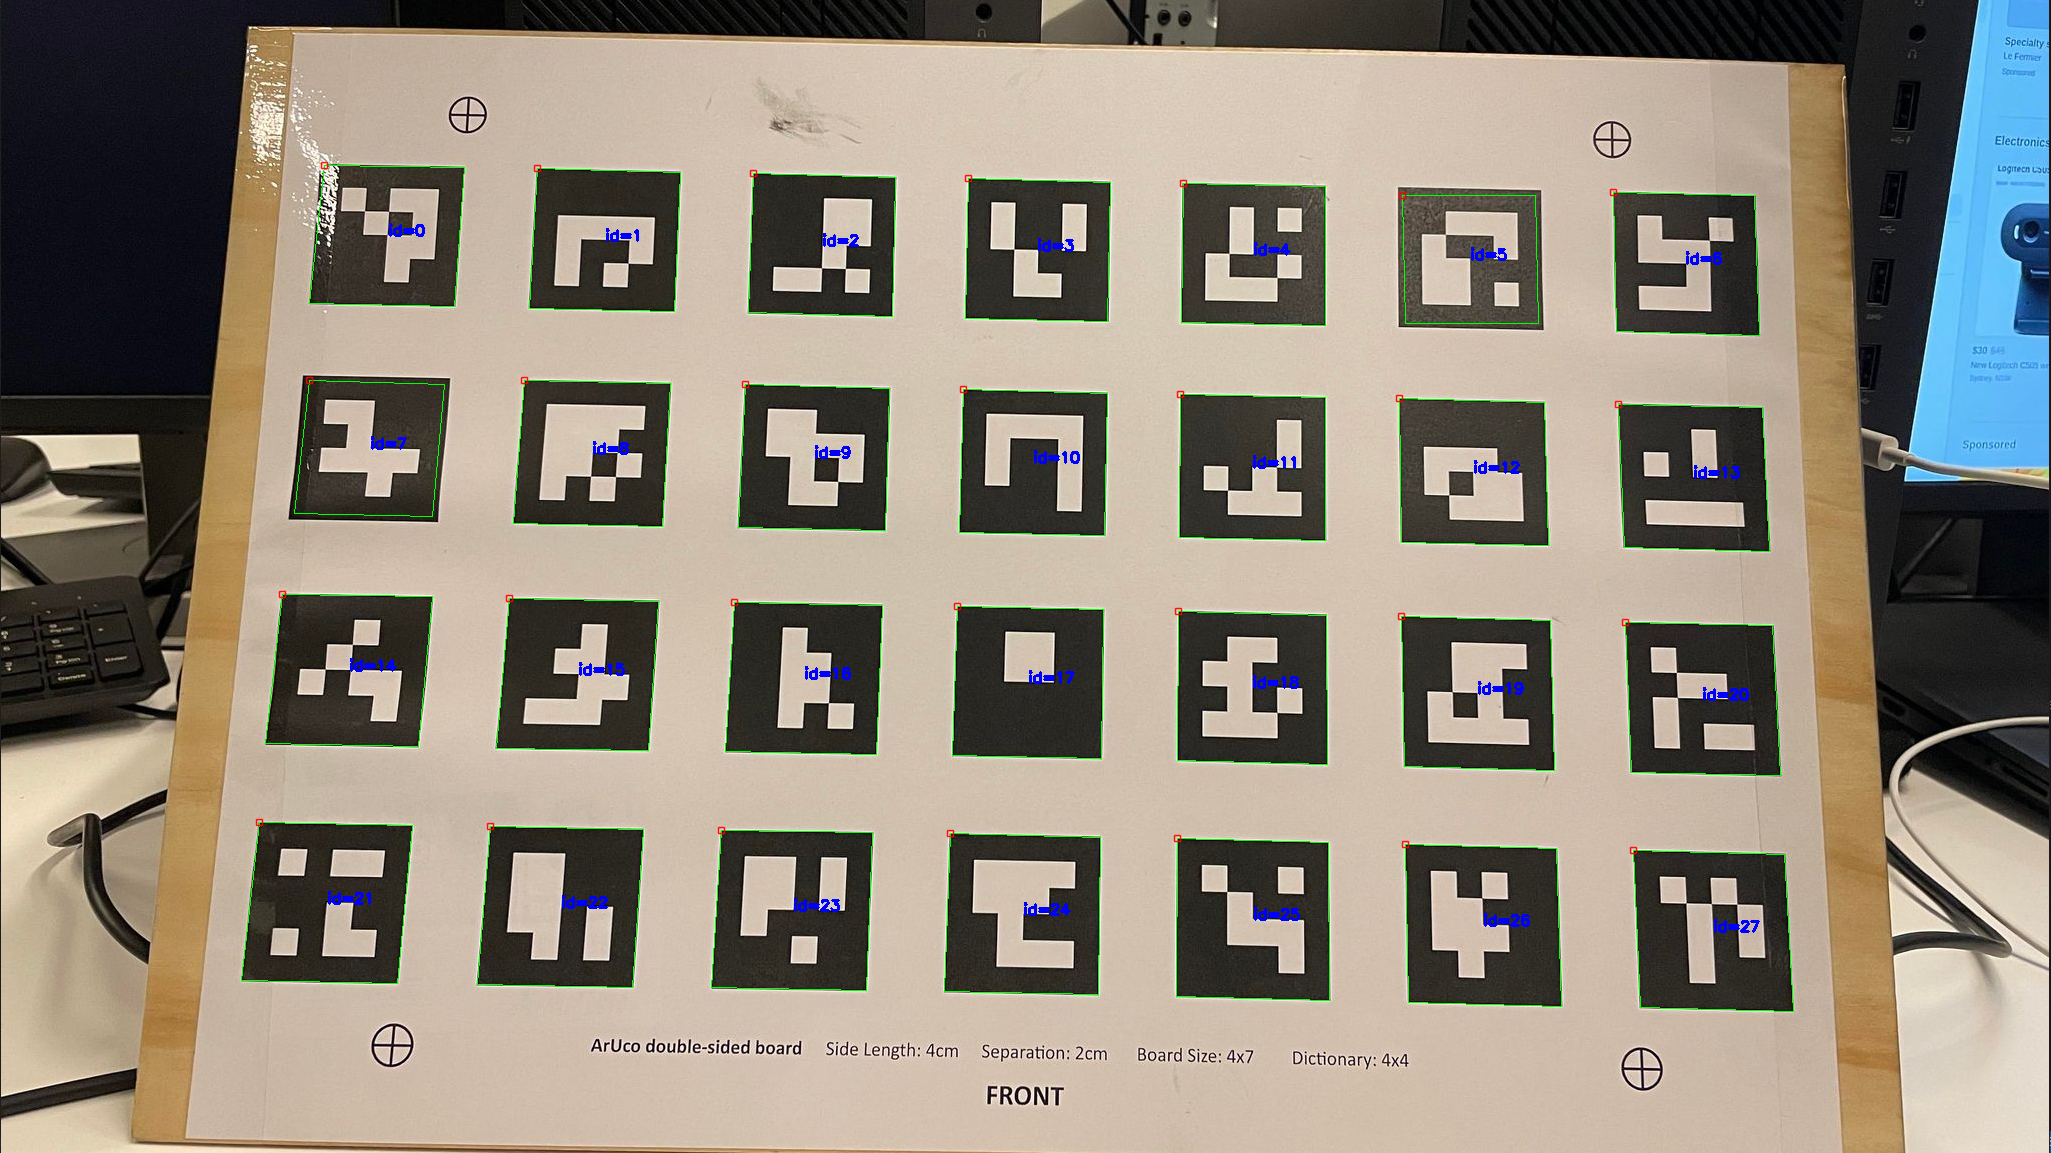
\includegraphics[width=1\textwidth]{Images/ArUco markers detection in image.png}
\caption{ArUco markers detection in image}
\end{figure}

After detecting markers and their IDs on the image, we have to determine their corresponding 3D points respected to ArUco board pose. As mentioned above (chapter 4.2), we already have had a list of markers' corner 3D coordinates (the object points) initialising by MATLAB. Based on the list of markers detected on the image and their IDs, we can define their relative 3D point coordinates in the board's origin frame (see Table \ref{tab:boardconfig}). Finally, after detecting the image points and the object points of ArUco markers, we should combine them with the intrinsic parameters of the respective camera (see Table \ref{tab:intrinsic}). Using the solvePnP() function, we can calculate the 3D rotation and translation vector from the ArUco board pose to the respective camera, and then estimate the relative pose between them. The demonstration of the ArUco board estimation process is shown below.

\begin{figure}[ht]
\centering
\includegraphics[width=0.7\textwidth]{Images/Board detection (front).jpg}
\caption{ArUco board estimation (front side)}
\end{figure}

\begin{figure}[ht]
\centering
\includegraphics[width=0.7\textwidth]{Images/Board detection (back).jpg}
\caption{ArUco board estimation (back side)}
\end{figure}

\clearpage
\section{Pose Graph Optimisation}
After estimating the relative pose between the double-sided ArUco board and each camera in the system, we separated the transformation into translation and rotation. The translation is presented as 3D vectors $[t_{x}, t_{y}, t_{z}]$, and the rotation is demonstrated as the quaternion formula $[q_{x}, q_{y}, q_{z}, q_{w}]$. We captured a total of 1652 images during the calibration process, which means each camera captured 413 photos of the ArUco board.

To implement the pose graph optimisation, we saved the estimated translation vectors and rotation quaternions of the whole calibration process as two CSV files: Nodes.csv and Edges.csv. 

One CSV file contained the nodes of the pose graph, including four nodes of cameras and 413 nodes of image poses. Camera 7 is the origin node, with the default value $[t_{x}, t_{y}, t_{z}] = [0, 0, 0]$ and $[q_{x}, q_{y}, q_{z}, q_{w}] = [0, 0, 0, 1]$. The remaining three camera nodes are the initial guess relative poses, which are measured directly from the multi-camera system. Finally, the image pose nodes are the transformations of the board's pose to the origin node, camera 7, which are estimated in the previous stage.

The other CSV file included the edges of the graph, which are the relative between nodes in the graph. We presented the edges between camera nodes and image pose nodes, which are the extrinsic parameters of each camera estimated from the ArUco board. In case the camera in our system could not detect the board, we used the last known pose of the previous detectable image. The edge values are also saved as 3D vectors $[t_{x}, t_{y}, t_{z}]$, and the rotation is demonstrated as the quaternion formula $[q_{x}, q_{y}, q_{z}, q_{w}]$.

\clearpage
\begin{figure}[ht]
\centering
\includegraphics[width=1\textwidth]{Images/CSV Nodes.png}
\caption{Nodes CSV file}
\end{figure}

In the Nodes.csv file, the rows list the nodes present in the pose graph and the transformation between the first node (node 7) and the corresponding node in this row. The columns describe the transformation components, including 3D translation vectors $[t_{x}, t_{y}, t_{z}]$ and rotation quaternion $[q_{x}, q_{y}, q_{z}, q_{w}]$. 

\clearpage
\begin{figure}[ht]
\centering
\includegraphics[width=0.9\textwidth]{Images/CSV Edges.jpg}
\caption{Edges CSV file}
\end{figure}

In the Edges.csv file, the first two columns represent two nodes of each edge, and the remaining columns are the relative poses between these two nodes.

\clearpage
After completing the two CSV files containing nodes and edges of the pose graph, we started the optimisation process. For testing purposes, we prepared a MATLAB script to run the pose graph optimisation algorithm because MATLAB can display the result as charts and histograms for easy follow-up. The MATLAB script reads the extrinsic parameters data set in the two CSV files, with the support of the Optimisation Toolbox of MATLAB, calculating the most optimal relative pose from more than 400 transformations between each camera and board's poses. The optimisation results are demonstrated in the figures below.

\begin{table}[ht]
    \caption{\label{tab:result}Pose Graph Optimisation result}
    \begin{tabular}{ |c|c|c|c|c|c|c|c| }
     \hline
    Cam & $t_{x}$ & $t_{y}$ & $t_{z}$ & $q_{x}$ & $q_{y}$ & $q_{z}$ & $q_{w}$ \\
     \hline
    7  & 0 & 0 & 0 & 0 & 0 & 0 & 1 \\ 
    8  & -0.3963  & -0.018545 & 0.0095207 & -0.0070655 & -0.0068763 & 0.0057706 & 0.99993 \\
    9  & -0.79415 & -0.025504 & 0.0021866 & -0.0070058 & -0.0088555 & 0.0090403 & 0.9999  \\ 
    10 & -1.0534  & -0.024433 & 0.17173   & -0.023018  & 0.25748    & 0.0039374 & 0.966   \\ 
     \hline
    \end{tabular}
    \begin{tabular}{|l|}
        Sum of residual error before optimising: 335.4759 (mm) \\
        Sum of residual error after optimising: 16.90129 (mm) \\
        \hline
    \end{tabular}
\end{table}

% \clearpage
\begin{figure}[ht]
\centering
\includegraphics[width=1\textwidth]{Images/optimised_pose_cameras.png}
\caption{\centering Poses of the optimised cameras and calibration board. Cam 7, which is coloured in red, is the origin. Every $10^{th}$ pose of the calibration board's origin represented by a 3D axis}
\end{figure}

\begin{figure}[ht]
\centering
\includegraphics[width=1\textwidth]{Images/graph_before_after_optimising.png}
\caption{\centering The pose graph before and after the optimisation is carried out. Blue circles are the nodes, red lines are the edges, and blue lines are loop-closure edges. The four camera nodes have been labelled in blue.}
\end{figure}

\chapter{Discussion}

\section{Accuracy}

Our approach covered in this capstone report consists of two main parts: proposing a double-sided ArUco board as the calibration target and applying General Graph Optimisation (G2O) to enhance the accuracy of the calibration result.

In terms of the double-sided ArUco board, experiments have shown that this approach worked well in our project scope. All 16 cameras in our system could thoroughly detect the double-sided ArUco board in their field of view, and then our program framework could estimate the board's poses which are respected to each camera. Moreover, Open-CV library's solvePnP() function can calculate the transformation that minimises the re-projection errors and guarantees accuracy of the calibration results. To improve the calibration result with our approach, we suggest increasing the number of ArUco markers on both sides as well as their dimension; the more ArUco tags captured and detected by the camera, the higher the accuracy of the relative pose estimated.

On the other hand, the final extrinsic parameters are also calculated very accurately after finishing the pose graph optimisation process. The residual errors for total edges of the pose graph before optimising is 335.4759 millimetres, being significantly reduced to 16.90129 millimetres after optimising. Considering our pose graph has a total number of 1849 edges, the average residual error is just 0.009 millimetres per edge. This value can be regarded as an acceptable error. If possible, we recommend increasing the number of nodes in the pose graph by capturing more images, and it will help enhance the result of the optimisation process.

\begin{figure}[h]
\centering
\includegraphics[width=1\textwidth]{Images/Board detection (both sides).jpg}
\caption{ArUco board estimation (both sides)}
\end{figure}

\begin{figure}[h]
\centering
\includegraphics[width=1\textwidth]{Images/Edge Residual Errors by Edge ID.png}
\caption{Edge Residual Errors by Edge ID}
\end{figure}

% \clearpage
% \section{Uncertainties and difficulties}
% The first difficulty we faced during working on this project was the synchronisation of the multiple camera system. Each camera in the system will capture images independently with a frequency of about 30 Hz, which means the interval between each shot is about 33 ms. To apply the General Graph Optimisation, we have to ensure that at least two cameras have captured the ArUco board at the same timestamp. Therefore, we had to deal with the synchronisation of the multi-camera system.


\clearpage
\section{Further works}

We have only demonstrated the calibration of four cameras, but the entire system contains sixteen. Complete calibration of all cameras requires synchronisation of images with the reference camera, which needs to be tested. Furthermore, increasing the number of cameras may affect the convergence of the optimisation and final accuracy of the calibration results. Testing will need to be carried out to exclude board poses with fewer edges, i.e. fewer cameras see the board in that pose.

Currently, there is no way of getting ground truth poses between the cameras with the physical camera system. Therefore, we can not quantitatively test the accuracy of the estimated poses from our method. It may be possible to set up a simulator with multiple cameras, where the pose between the cameras is known, to test the calibration procedure. Noise can be added to images to replicate the functionality of physical cameras. Our calibration approach could also be tested with existing methods to compare results.

An important quantity that has not been considered is the uncertainty of our calibration parameters arising from the propagation of sensor noise. The calibration method relies on detecting fiducial markers in noisy images of the calibration board. The corners, in pixel coordinates, that are used in the optimisation will have some associated uncertainty. This uncertainty will be carried through the estimation of the board poses, and through the graph-based optimisation. Estimating the uncertainty can help us to understand the reliability of the final calibrated parameters, and potentially guide the collection of new images from cameras with high uncertainty. In completing this task, there is a possibility to publish the findings to a research conference.

Additionally, we would like to integrate the Pose Graph Optimisation into our program framework, so we will not need to save the relative pose between the ArUco board and each camera to CSV files, then run the MATLAB script for the optimisation. The General Graph Optimisation (G2O) algorithm will be coded in C++ and directly integrated into our framework, and then the optimisation process will be automatically run after finishing the board detection process for each camera. Besides, we would like to modify our program framework to be more modular to improve the processing speed and efficiency of the program. We will publish our framework in a public repository on GitHub and as an open-source ROS package for users.

\chapter{Conclusion}
In conclusion, this capstone report proposes an approach for camera calibration of multiple partially overlapping cameras to determine the extrinsic parameters of the camera system. This project is a part of the "Objective real-time live cattle assessments to improve profit" funded project by Meat and Livestock Australia.

As a part of camera calibration, this report proposes to use an augmented planar board as the calibration target. A double-sided planar board with ArUco markers is employed to solve the problem with cameras facing each other and having overlapping fields of view. In addition, the General Graph Optimisation (G2O) is applied to optimise the calibration results. Experiments were also implemented to test the approach's feasibility, and the results obtained were also very encouraging. However, this method still needs improvement to increase efficiency and accuracy.

In the future, the program framework, as well as the algorithm, would be improved to test with the whole 16 cameras of this system. We would intend to publish our approach as a ROS package and store it on a public repository on GitHub for further development. 



%%%%%%%%%%%%%%%%%%%%%%%%%%%%
% BIBLIOGRAPHY
\clearpage
\phantomsection
\addcontentsline{toc}{chapter}{Bibliography}
\bibliographystyle{uts.bst}
\bibliography{Bibliography/capstone_references}
%%%%%%%%%%%%%%%%%%%%%%%%%%%%


%%%%%%%%%%%%%%%%%%%%%%%%%%%%
% START APPENDICES
\appendix
%%%%%%%%%%%%%%%%%%%%%%%%%%%%


% %-----------------------------------------------------
% % Appendix: Code
% %-----------------------------------------------------
% \chapter{Code}
% \label{app:code}

% \begin{verbatim}
% 10 PRINT "HELLO WORLD"
% \end{verbatim}

% \input{Chapters/appendix1.tex}


%%%%%%%%%%%%%%%%%%%%%%%%%%%%
% END DOCUMENT
\end{document}
%%%%%%%%%%%%%%%%%%%%%%%%%%%%
